\tikzstyle{vertex}=[circle,fill=black,minimum size=10pt]
\tikzstyle{edge} = [draw,line width=2pt]
\tikzstyle{green edge} = [draw,line width=2pt,green]
\tikzstyle{blue edge} = [draw,line width=2pt,blue]
\tikzstyle{red edge} = [draw,line width=2pt,red]
\tikzstyle{grey edge} = [draw,line width=2pt,yellow]

\begin{figure}
  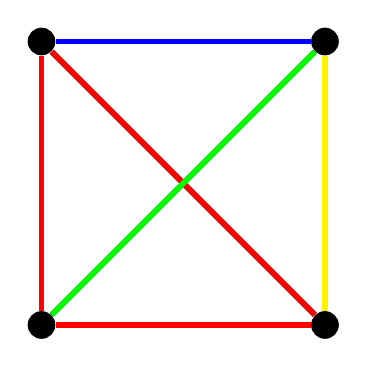
\begin{tikzpicture}[scale=1.8, auto,swap]
    \foreach \pos/\name in { {(0,0)/a},{(0,2)/b},{(2,0)/c},{(2,2)/d}} % Erstes Quadrat
    \node<1->[vertex] (\name) at \pos {};
    % Connect vertices with edges and draw weights
    \foreach \source/ \dest in {a/b,a/c,a/d,b/c,b/d,c/d}
    \path<1->[edge] (\source) --  node{}  (\dest);
%
%    % Start animating the vertex and edge selection. 

    \foreach \source/ \dest in {a/b,a/c,b/c}
    \path<2->[red edge] (\source) --  node{}  (\dest);
    \foreach \source/ \dest in {a/d}
    \path<3->[green edge] (\source) --  node{}  (\dest);
    \foreach \source/ \dest in {b/d}
    \path<4->[blue edge] (\source) --  node{}  (\dest);
    \foreach \source/ \dest in {c/d}
    \path<5->[grey edge] (\source) --  node{}  (\dest);

%    % For convenience we use a background layer to highlight edges
%    % This way we don't have to worry about the highlighting covering
%    % weight labels. 
%    %\begin{pgfonlayer}{background}
%    %    \pause
%    %    \foreach \source / \dest in {d/a,d/f,a/b,b/e,e/c,e/g}
%    %        \path<+->[selected edge] (\source.center) -- (\dest.center);
%    %    \foreach \source / \dest / \fr in {d/b/4,d/e/5,e/f/5,b/c/6,f/g/7}
%    %        \path<\fr->[ignored edge] (\source.center) -- (\dest.center);
%    %\end{pgfonlayer}
  \end{tikzpicture}
\end{figure}
